\documentclass[article]{jss}

\usepackage{amsmath,booktabs,graphicx,lmodern,placeins}

\author{Oluwajuwon Mayomi Akanbi\\Independent Researcher / Developer}
\Plainauthor{Oluwajuwon Mayomi Akanbi}
\title{\pkg{systemgmmkit}: Reproducible Dynamic-Panel GMM Workflows in \proglang{Python}}
\Plaintitle{systemgmmkit: Reproducible Dynamic-Panel GMM Workflows in Python}
\Shorttitle{\pkg{systemgmmkit}: Dynamic-Panel GMM Workflows}
\Abstract{
\pkg{systemgmmkit} is a \proglang{Python} toolkit for static panel estimators, instrumental-variable
estimation, Difference GMM, System GMM, diagnostics, post-estimation, panel-aware validation, forecasting, and
diagnostic-constrained specification search. The package does not introduce a new GMM estimator. Its
contribution is an integrated and auditable workflow in which model specification, instrument construction,
finite-sample covariance choices, diagnostics, predictions, and reporting remain visible. This paper documents
release 1.0.0, including structured instrument-health reporting and the six-specification numerical
certificate established in release 0.5.14 against \proglang{Stata}
\code{xtabond2}, nested leakage-controlled N-CMAPSS results, an executed automatic GMM search, and Universal Output
Hub table generation. The reported parity is benchmark-specific and must not be read as evidence that every
empirical specification is valid.
}
\Keywords{dynamic panel data, generalized method of moments, System GMM, \proglang{Python}, reproducibility}
\Plainkeywords{dynamic panel data, generalized method of moments, System GMM, Python, reproducibility}
\Address{
Oluwajuwon Mayomi Akanbi\\
Independent Researcher / Developer\\
URL: \url{https://github.com/Akanom/systemgmmkit}
}

\begin{document}

\section{Introduction}
Dynamic-panel models are used when outcomes are persistent, unit-specific effects matter, and one or more
regressors may be predetermined or endogenous \citep{arellano1991some,blundell1998initial,bond2002dynamic}.
In practice, applied work requires more than a coefficient vector. Researchers must control the estimation
sample, define instrument roles and lag windows, monitor instrument growth, assess serial-correlation and
over-identification diagnostics, and preserve enough metadata for independent reproduction.

\pkg{systemgmmkit} brings these tasks into a common \proglang{Python} interface. The package covers OLS, pooled OLS,
fixed effects, random effects, panel IV/2SLS, Difference GMM, and System GMM, with structured result objects and
post-estimation utilities. It complements established software rather than ranking or replacing it
\citep{roodman2009xtabond2,croissant2008panel,seabold2010statsmodels,sheppard2024linearmodels,pydynpd}.

\section{Software design and claim boundaries}
The public workflow separates model specification, estimation, diagnostics, prediction, and reporting. For
dynamic GMM, users declare the dependent variable, panel indexes, regressor roles, lag windows,
transformation, collapsed or uncollapsed instruments, estimation step, and covariance correction. Results
retain observation and group counts, instrument counts, coefficient and covariance output, Hansen and Sargan
tests, and Arellano--Bond serial-correlation diagnostics.

Version 1.0.0 declares the documented public interface stable and adds a structured instrument-health
assessment to native and \code{pydynpd} result summaries. It reports instrument and group counts, their
ratio, and conservative acceptable, approaching, critical, or unavailable states. A critical state means
that instruments outnumber groups and prompts shorter lag windows, collapsed instruments, and sensitivity
checks. This rule is a screening signal rather than proof of bias or automatic invalidation of Hansen/Sargan
inference.

Release 0.5.14 added certified unbalanced-panel and variable-specific missing-data paths to the maintained
\code{xtabond2} evidence. The release certificate tests complete parameter sets, Windmeijer-corrected
two-step standard errors, counts, diagnostics, and, where relevant, exact estimation-sample keys. Agreement is
therefore asserted only for the registered benchmark specifications. A passing parity row says that two
implementations agree; it does not say that the instruments are substantively valid or that the specification
answers a particular research question.

\section{Econometric formulation}
The package represents the dynamic panel model as
\begin{equation}
\label{eq:dynamic-panel}
y_{it}
= \rho y_{i,t-1}
+ \mathbf{x}_{it}^\top \boldsymbol{\beta}
+ \alpha_i + \tau_t + \varepsilon_{it},
\end{equation}
where $i=1,\ldots,N$ indexes units, $t=1,\ldots,T_i$ indexes time,
$\alpha_i$ is an unobserved unit effect, and $\tau_t$ is an optional time effect.
The regressor vector $\mathbf{x}_{it}$ is partitioned by the user's endogenous,
predetermined, and exogenous declarations. Setting $\rho=0$ yields the static-panel
core; the role declarations and lag windows determine the dynamic-GMM instrument design.

First differencing removes the time-invariant unit effect:
\begin{equation}
\label{eq:first-difference}
\Delta y_{it}
= \rho\,\Delta y_{i,t-1}
+ \Delta\mathbf{x}_{it}^\top\boldsymbol{\beta}
+ \Delta\tau_t + \Delta\varepsilon_{it}.
\end{equation}
For a variable $z$ assigned a GMM-style role, Difference GMM uses level instruments
whose admissible lags are recorded explicitly by the role- or variable-specific set
$\mathcal{L}_z^D$:
\begin{equation}
\label{eq:difference-moments}
\operatorname{E}\!\left[z_{i,t-s}\,\Delta\varepsilon_{it}\right]=0,
\qquad s\in\mathcal{L}_z^D.
\end{equation}
For the lagged dependent variable, the conventional lower bound is two. System GMM
stacks Equation~\ref{eq:first-difference} with the level equation and, under the
additional initial-condition restrictions of \citet{blundell1998initial}, admits
level-equation moments of the form
\begin{equation}
\label{eq:system-moments}
\operatorname{E}\!\left[\Delta z_{i,t-1}
  \left(\alpha_i+\varepsilon_{it}\right)\right]=0.
\end{equation}
Thus the implementation constructs $Z_i$ from declared roles and lag windows rather
than silently selecting instruments. With $\boldsymbol{\theta}=(\rho,\boldsymbol{\beta}^\top)^\top$,
the one- or two-step estimator minimizes
\begin{equation}
\label{eq:gmm-objective}
\begin{aligned}
\mathbf{g}_N(\boldsymbol{\theta})
  &= \frac{1}{N}\sum_{i=1}^N Z_i^\top
     \mathbf{u}_i(\boldsymbol{\theta}), \\
\widehat{\boldsymbol{\theta}}
  &= \underset{\boldsymbol{\theta}}{\operatorname{arg\,min}}\;
     \mathbf{g}_N(\boldsymbol{\theta})^\top
     \widehat{W}_N
     \mathbf{g}_N(\boldsymbol{\theta}).
\end{aligned}
\end{equation}
For two-step estimation, $\widehat{W}_N$ is updated from first-step residual moments;
the Windmeijer adjustment changes the reported finite-sample covariance, not the point
estimate. For an overidentified model with $q$ instruments and $k$ estimated parameters,
the robust Hansen statistic is
\begin{equation}
\label{eq:hansen}
J_N
= N\,\mathbf{g}_N(\widehat{\boldsymbol{\theta}})^\top
  \widehat{W}_N
  \mathbf{g}_N(\widehat{\boldsymbol{\theta}})
\;\overset{a}{\sim}\;\chi^2_{q-k}.
\end{equation}
This reference distribution requires valid moment conditions and regularity conditions.
Accordingly, Hansen non-rejection and AR(2) non-rejection are reported as diagnostics,
not treated as proofs of identification.

\section{Reproducible output workflow}
All tables and figures in this manuscript are generated from machine-readable artifacts. \pkg{Universal Output
Hub} 0.2.4 is the single manuscript table exporter. The numerical chain is raw or controlled data, executable
model code, normalized CSV or release certificate, OutputHub LaTeX fragment or scripted figure, and finally
this document. All stochastic procedures use the fixed seed 20260724. Debug output,
row-level panel previews, API snapshots, smoke-test status tables, duplicate manual renderings, and stale
deterministic target-lag results are retained outside the manuscript or excluded entirely.

\section{Leakage-controlled N-CMAPSS application}
The N-CMAPSS DS01 development data are used as a compact application of panel preparation and late-cycle
validation. Remaining useful life decreases deterministically with cycle, so including lagged RUL---or the
derived lagged risk proxy---creates a tautological prediction problem. The revised design removes those target
lags. It retains a lagged-sensor OLS baseline and adds a nonlinear direct sensor model whose scaler, principal
components, and tuning are fitted only on training windows (Table~\ref{tab:application-design}).

Let $\mathbf{s}_{it}$ denote the raw sensor vector and let $\mathcal{P}_\mathcal{T}$
denote scaling followed by principal-component analysis fitted only on training window
$\mathcal{T}$. The nonlinear predictor used in the final holdout comparison is
\begin{equation}
\label{eq:ncmapss-predictor}
\begin{aligned}
\mathbf{q}_{it} &= \mathcal{P}_\mathcal{T}(\mathbf{s}_{it}), \\
\widehat{r}_{it}
  &= f_{\widehat{\eta}}\!\left(
     \mathbf{q}_{it},\mathbf{q}_{i,t-1},
     \Delta\mathbf{q}_{it},\overline{\mathbf{q}}_{it}^{(3)}
     \right),
\end{aligned}
\end{equation}
where $r_{it}$ is the risk proxy and $f_{\widehat{\eta}}$ is the selected random
forest. Equation~\ref{eq:ncmapss-predictor} contains no cycle, lagged RUL, or lagged
risk term and is a predictive mapping rather than a structural or causal equation.

\begin{table}[t!]
\centering
\small
\setlength{\tabcolsep}{4.5pt}
\renewcommand{\arraystretch}{1.16}
\input{tables/table_01_application_design.tex}
\caption{\label{tab:application-design} Leakage-controlled N-CMAPSS application design. Source: Author's computation from the processed N-CMAPSS DS01 panel (Artifacts 01 and 05). Notes: The target is a risk proxy derived from RUL. Lagged risk and lagged RUL are excluded because they encode a deterministic countdown identity.}
\end{table}


Table~\ref{tab:application-estimates} reports pooled and unit fixed-effects baselines. The lagged sensor-state
coefficient is positive in both models (0.032 and 0.028) and is distinguishable from zero at the 5 percent level.
The health-setting coefficient is negative and stable across specifications. By contrast, the flow-control
coefficient is positive in pooled OLS but becomes small and statistically indistinguishable from zero after unit
effects are introduced. In-sample fit rises only modestly, from 0.584 to 0.604, which is consistent with some
unit heterogeneity but does not establish predictive generalization.

\begin{table}[t!]
\centering
\small
\setlength{\tabcolsep}{4.5pt}
\renewcommand{\arraystretch}{1.16}
\input{tables/table_02_application_estimates.tex}
\caption{\label{tab:application-estimates} N-CMAPSS lagged-sensor baseline estimates. Source: Author's computation using statsmodels with HC1 covariance (Artifacts 02 and 03). Notes: HC1 standard errors are in parentheses. Unit fixed effects are included in the second column but their individual coefficients are omitted from display.}
\end{table}


\FloatBarrier

The late-cycle comparison withholds cycles 71--100 (Table~\ref{tab:holdout}). The pooled lagged-sensor baseline
has RMSE 0.332 and out-of-sample $R^2$ -15.783; its squared error exceeds
that of a constant benchmark equal to the observed holdout mean. The direct random forest instead attains RMSE
0.071, MAE 0.053, SMAPE 0.062, and $R^2$
0.232. Candidate selection uses three expanding windows entirely within cycles 1--70, and
the scaler and PCA are refitted in every training window before the final outer evaluation. The improvement is
predictive evidence for this split, not a causal claim or proof that late-life distribution shift is absent.

\begin{table}[t!]
\centering
\small
\setlength{\tabcolsep}{4.5pt}
\renewcommand{\arraystretch}{1.16}
\input{tables/table_03_holdout_performance.tex}
\caption{\label{tab:holdout} Late-cycle holdout performance. Source: Author's computation from the nested cycle-ordered validation (Artifacts 04, 06, and 07). Notes: The forest is selected only within cycles 1--70 using expanding windows. The final cycles 71--100 are evaluated once; neither model uses lagged risk, lagged RUL, or cycle.}
\end{table}


\FloatBarrier

\section{Controlled dynamic-GMM results}
The controlled panel contains 120 units observed over ten periods. The data-generating coefficients are 0.55
for persistence, 0.35 for the predetermined regressor, and 0.25 for the exogenous regressor. Both estimators use
collapsed instruments and two-step covariance calculations. Instrument counts (five and eight) remain well
below the number of groups.

The exact controlled data-generating process is
\begin{equation}
\label{eq:controlled-dgp}
y_{it}
= 0.55y_{i,t-1} + 0.35x_{it}^{\mathrm{pred}}
+ 0.25x_{it}^{\mathrm{exog}}
+ \alpha_i + \tau_t + \varepsilon_{it}.
\end{equation}
The predetermined regressor depends on the previous-period disturbance but not the
current disturbance; the exogenous regressor is generated independently.

Difference GMM estimates the exogenous effect at 0.251, close to its generating value, while its persistence
estimate is 0.711 with a comparatively large standard error. System GMM estimates the exogenous effect at 0.242
but produces a higher persistence estimate (0.929) and a weak predetermined-regressor estimate (0.056). These
differences show why estimator choice cannot be reduced to in-sample precision. In this controlled realization,
System GMM is not uniformly closer to the generating parameters.

Both models show the expected first-order serial correlation after differencing and do not reject AR(2) at
conventional levels. Hansen p-values are 0.503 and 0.794. These diagnostics are compatible with the maintained
instrument design, but non-rejection is not proof of instrument exogeneity and a high Hansen p-value can be
uninformative when instruments proliferate \citep{roodman2009xtabond2}.

\begin{table}[t!]
\centering
\small
\setlength{\tabcolsep}{4.5pt}
\renewcommand{\arraystretch}{1.16}
\input{tables/table_04_controlled_gmm_results.tex}
\caption{\label{tab:controlled-gmm} Controlled Difference GMM and System GMM results. Source: Author's computation with systemgmmkit 1.0.0 (Artifact 22). Notes: Two-step collapsed specifications. Standard errors are in parentheses. AR and over-identification entries are p-values; diagnostic non-rejection is not proof of validity.}
\end{table}


\section{Cross-software validation}
The formal System GMM evidence in release 0.5.14 comprises six collapsed two-step specifications. Across them,
native and \proglang{Stata} results have identical observation, group, instrument, and over-identification counts. Maximum
absolute coefficient differences are below the registered $10^{-6}$ tolerances, and relative standard-error
differences remain within each specification's registered tolerance (Table~\ref{tab:parity-parameters}).
The unbalanced and variable-missing fixtures also match exact panel-time estimation-sample keys.

\begin{table}[t!]
\centering
\small
\setlength{\tabcolsep}{4.5pt}
\renewcommand{\arraystretch}{1.16}
\begin{tabular}{lccccccc}
\toprule
Specification & N & Groups & Instr. & Max coef. diff & Max rel. SE diff & Keys & Status \\
\midrule
Baseline controls & 1248 & 96 & 8 & 2.31e-14 & 5.78e-07 & Not required & PASS \\
No controls & 1248 & 96 & 7 & 8.88e-16 & 5.46e-07 & Not required & PASS \\
Three-way controls & 1248 & 96 & 16 & 3.66e-15 & 2.63e-06 & Not required & PASS \\
Decomposition controls & 1248 & 96 & 12 & 1.89e-14 & 1.57e-07 & Not required & PASS \\
Unbalanced panel & 1174 & 96 & 8 & 1.04e-14 & 1.54e-06 & Exact & PASS \\
Variable missingness & 1216 & 96 & 8 & 2.29e-14 & 2.16e-06 & Exact & PASS \\
\bottomrule
\end{tabular}
\caption{\label{tab:parity-parameters} System GMM parameter and count parity with Stata xtabond2. Source: Author's computation from the signed v0.5.14 release certificate (Artifact 24). Notes: All six release-certified specifications pass their registered tolerances. Exact sample-key matching is required for the unbalanced and variable-missing designs; Not required means that gate was not registered for the four balanced fixtures.}
\end{table}


Table~\ref{tab:parity-diagnostics} separates numerical agreement from empirical adequacy. Baseline and
unbalanced designs do not reject the over-identifying restrictions at 5 percent, whereas several deliberately
maintained fixtures do. Those rejections are preserved because a parity test must reproduce the comparator's
result even when the specification would not be selected for substantive use. AR(2) is not rejected in any of
the six registered specifications.

\begin{table}[t!]
\centering
\small
\setlength{\tabcolsep}{4.5pt}
\renewcommand{\arraystretch}{1.16}
\begin{tabular}{lcccccc}
\toprule
Specification & Hansen p & Sargan p & AR(1) p & AR(2) p & Over-id (5\%) & Status \\
\midrule
Baseline controls & 0.160 & 0.088 & 0.080 & 0.868 & Do not reject & PASS \\
No controls & 0.024 & 0.006 & 0.136 & 0.920 & Reject & PASS \\
Three-way controls & 0.021 & 0.000 & 0.000 & 0.990 & Reject & PASS \\
Decomposition controls & 0.006 & 0.000 & 0.064 & 0.152 & Reject & PASS \\
Unbalanced panel & 0.232 & 0.297 & 0.107 & 0.873 & Do not reject & PASS \\
Variable missingness & 0.012 & 0.001 & 0.033 & 0.111 & Reject & PASS \\
\bottomrule
\end{tabular}
\caption{\label{tab:parity-diagnostics} System GMM diagnostic parity with Stata xtabond2. Source: Author's computation from the signed v0.5.14 release certificate (Artifact 24). Notes: PASS denotes cross-software numerical agreement. The over-identification column reports the Stata-side 5 percent decision and is not a model endorsement.}
\end{table}


Static reference checks tell a similarly qualified story. OLS, pooled OLS, and fixed-effects results agree
numerically with aligned \proglang{Python}/\proglang{R} references and closely with \proglang{Stata} exports. Random-effects and 2SLS
coefficients also agree, but standard errors vary modestly under package-specific covariance conventions.
Table~\ref{tab:static-reference} therefore labels those rows as coefficient agreement rather than overstating
full covariance parity.

\begin{table}[t!]
\centering
\small
\setlength{\tabcolsep}{4.5pt}
\renewcommand{\arraystretch}{1.16}
\input{tables/table_07_static_reference_checks.tex}
\caption{\label{tab:static-reference} Aligned static-estimator reference checks. Source: Author's computation from the v0.5.14 cross-software checks (Artifact 27). Notes: Specifications and samples are aligned. Random-effects and 2SLS claims remain at the coefficient level because covariance conventions differ across packages.}
\end{table}


\section{Post-estimation, ML-style workflows, and automatic GMM search}
The ML namespace is an orchestration layer around fitted econometric results. It supplies panel-aware splitting,
prediction metrics, model comparison, forecasting, and expanding-window backtesting. These tools help distinguish
estimation fit from predictive performance, but predictive accuracy does not create causal identification
\citep{roberts2017crossvalidation,bergmeir2018note,cerqueira2019evaluating}.

The automatic GMM search layer explores user-declared Difference/System GMM candidates over lag windows,
transformation, estimation step, collapse choice, and related options. Candidate ranking occurs only after
diagnostic gates for convergence, AR(2), Hansen behavior, and instrument proliferation. This design reduces
mechanical specification shopping, but it cannot supply substantive exclusion restrictions or decide which
moment conditions are credible. The final specification remains a research decision.

For the executed strict-policy search, the diagnostic filter and predictive selection
can be summarized as
\begin{equation}
\label{eq:auto-search}
\begin{aligned}
\mathcal{A}
  &= \left\{m\in\mathcal{M}:\,
     \mathrm{fit}_m=\mathrm{ok},\,
     0.05<p_{H,m}<0.99,\,
     p_{\mathrm{AR}(2),m}>0.05,\,
     j_m\le n_m\right\}, \\
\widehat{m}
  &= \underset{m\in\mathcal{A}}{\operatorname{arg\,min}}\;
     \operatorname{RMSE}_m.
\end{aligned}
\end{equation}
Here $j_m$ and $n_m$ are the instrument and group counts. Missing required diagnostics
exclude a candidate under the strict policy. These thresholds are configurable API
defaults and should not be interpreted as universal statistical decision rules.

\begin{table}[t!]
\centering
\small
\setlength{\tabcolsep}{4.5pt}
\renewcommand{\arraystretch}{1.16}
\begin{tabular}{lcccccc}
\toprule
Candidate & Status & RMSE & R2 & Hansen p & AR(2) p & Instr. \\
\midrule
System, 2:2 & Selected & 0.602 & 0.923 & 0.669 & 0.287 & 6 \\
System, 2:3 & Admissible & 0.606 & 0.922 & 0.929 & 0.286 & 8 \\
Difference, 2:2 & Rejected & 1.877 & 0.251 & Not reported & 0.139 & 3 \\
Difference, 2:3 & Admissible & 1.382 & 0.594 & 0.897 & 0.151 & 5 \\
\bottomrule
\end{tabular}
\caption{\label{tab:auto-search} Diagnostic-first automatic GMM search on the controlled panel. Source: Author's computation from the executed diagnostic-first search. Notes: Cycle-ordered holdout covers the final two periods. The strict gate rejects the Difference GMM 2:2 candidate because a Hansen test is not reported; the value is not imputed. Selection ranks only admissible candidates and does not establish causal identification.}
\end{table}


The executed four-candidate search selects the System GMM 2:2 lag window. Its cycle-ordered holdout RMSE is
0.602 and its out-of-sample $R^2$ is 0.923. The System GMM 2:3 candidate is also admissible and performs
similarly, while the admissible Difference GMM 2:3 candidate has a markedly larger RMSE of 1.382. The
Difference GMM 2:2 candidate is rejected by the strict gate because its exactly identified design does not
provide a Hansen test. This is a policy choice for comparable diagnostic screening, not evidence that every
exactly identified model is intrinsically invalid.

A repository-only comparison artifact places this selected candidate beside external \proglang{Python}
predictive baselines on the identical final-two-period holdout. The \pkg{statsmodels} OLS baseline records
RMSE 0.597 and $R^2$ 0.924; the
\pkg{scikit-learn} random forest records RMSE 0.655 and $R^2$
0.909. The artifact is not reproduced as a manuscript table. It checks temporal-split and
predictive-metric behavior only, not estimator parity, Hansen/AR agreement, or causal identification.

\begin{figure}[t!]
\centering
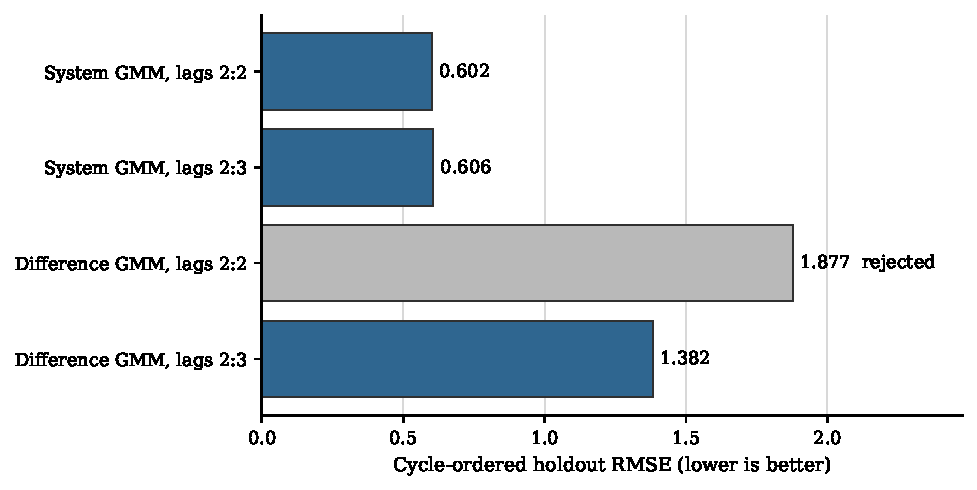
\includegraphics[width=0.88\textwidth]{figures/01_auto_gmm_search_holdout.pdf}
\caption{\label{fig:auto-search} Cycle-ordered holdout error for the four automatic GMM-search candidates.
Source: Author's computation from the executed search in Table~\ref{tab:auto-search}. The gray candidate
failed the strict diagnostic-availability gate; lower RMSE is
better, and predictive ranking does not establish causal identification.}
\end{figure}

\begin{table}[t!]
\centering
\small
\setlength{\tabcolsep}{4.5pt}
\renewcommand{\arraystretch}{1.16}
\begin{tabular}{lccc}
\toprule
Layer & APIs/workflow & Runtime & Boundary \\
\midrule
Post-estimation & predict, confint, margins & API verified & Estimator-based inference \\
Panel validation & split, metrics & Smoke passed & Panel-time order \\
Forecasting & forecast, backtest, compare & API verified & No causal claim \\
\bottomrule
\end{tabular}
\caption{\label{tab:workflow-layer} Post-estimation and ML-style workflow coverage. Source: Author's runtime audit of the installed systemgmmkit 1.0.0 API. Notes: This is workflow coverage, not estimator parity. Prediction and validation utilities operate around fitted econometric results and do not create causal identification.}
\end{table}


\section{Limitations}
The N-CMAPSS illustration has only six units after processing and is too small to serve as a formal dynamic-GMM
application. It is retained to demonstrate leakage control and honest temporal validation. The controlled GMM
exercise is synthetic and establishes workflow behavior, not external validity. Cross-software certificates are
specification-specific, and their tolerances, samples, comparator versions, and provenance must accompany any
parity claim. Finally, no diagnostic or automated search rule can replace an argument for identification.

% AUTHOR-LED SECTION: add the field-specific literature synthesis, substantive application
% motivation, broader interpretation, and final conclusion here after independent reading.

\section{Availability and reproducibility}
The source code and release evidence are available from the project repository under the MIT license. The
separate JOSS paper remains in \code{paper/paper.md}. This JSS manuscript and its OutputHub-generated tables
live only in \code{paper\_jss/}. Running \code{run\_all.py} in open mode
recreates data products, model outputs, comparisons, all nine tables, the figure, the manuscript PDF, logs,
checksums, and the reproducibility manifest. The build refuses to run unless the installed package is exactly
version 1.0.0 and the table exporter is exactly \pkg{Universal Output Hub} 0.2.4. The six-specification parity
tables are read from the signed \code{v0.5.14} Git tag rather than from mutable development artifacts.
The portable manual Stata script and the repository-only external Python comparison are retained under
\code{replication/scripts/} with machine-readable outputs for future independent review.

\section*{AI assistance disclosure}
Generative AI tools assisted with software workflow planning, code review, table-pipeline construction, and
drafting/editing of technical prose. The author is responsible for verifying every result, revising the text,
completing the literature-led discussion, and ensuring that the submitted manuscript satisfies journal policy.

\bibliography{../paper/paper}

\end{document}
